\section{Data and noise model}\label{sec:data}

\subsection{Selection of the data}
The data are LIGO-Hanford (H1) strain at 4096\,Hz from O1 (September 2015--January 2016), downloaded with \texttt{GWpy}~\cite{gwpy} from GWOSC. Eight chunks of 4096\,s were selected, evenly spread over the run, fully inside the
H1 science segments and at least 2000\,s from every catalogued event (GW150914, GW151012, GW151226 and the two candidates); the closest chunk is more than $1.7\times10^5$\,s from an event, so the chunks can be treated as noise only.
Table~\ref{tab:chunks} lists them with the train/validation/test assignment. The split is made \emph{by chunk}, interleaved in time so that each part samples the whole run, never by window: neighbouring windows share noise.
The test chunks (3 and 7, Nov.\ 2015 and Jan.\ 2016) therefore come from detector epochs, PSDs and glitch conditions that no threshold or model has seen.

\begin{table}[h]\centering\small
\begin{tabular}{rllr}
\toprule
chunk & start (UTC) & split & windows\\
\midrule
0 & 2015-09-12 06:59 & train & 4056\\
1 & 2015-10-04 16:01 & val & 4056\\
2 & 2015-10-19 13:17 & train & 4056\\
3 & 2015-11-07 23:46 & \textbf{test} & 4056\\
4 & 2015-11-28 01:03 & train & 4056\\
5 & 2015-12-16 19:37 & val & 4056\\
6 & 2015-12-31 06:38 & train & 4056\\
7 & 2016-01-19 13:43 & \textbf{test} & 4056\\
\bottomrule
\end{tabular}
\caption{The eight H1 chunks (4096\,s each). Windows are the non-overlapping one-second analysis windows left after removing 20\,s at each end.}\label{tab:chunks}
\end{table}

\subsection{PSD, whitening and analysis windows}
The noise power spectral density $S_n(f)$ of each chunk is estimated with Welch's method~\cite{Welch} (4\,s Hann segments, 0.25\,Hz resolution) using the \emph{median} average, which is robust to glitches.
Each chunk is whitened with its own PSD, band-passed to $30$--$500\Hz$ and down-sampled to 1024\,Hz (the band is below the new Nyquist frequency, so no information is lost), then cut into non-overlapping windows
of one second (1024 samples). One window is the unit of every later analysis. In the frequency domain a window has bins $V_k=\mathrm{rfft}(v)_k/\sqrt{512}$ at 1\,Hz spacing; for stationary Gaussian noise $\mathrm{Re}\,V_k$ and $\mathrm{Im}\,V_k$
are independent $\mathcal N(0,1)$ in the band, so that the inner product of two signals is $\langle a,b\rangle=\mathrm{Re}\sum_k A_kB_k^*$ and the optimal SNR is
\begin{equation}
\snr^2=\langle h,h\rangle=4\int\frac{|\tilde h(f)|^2}{S_n(f)}\,df .\label{eq:snr}
\end{equation}
Figure~\ref{fig:asd} shows the amplitude spectral density of the eight chunks: the shape is stable, the in-band sensitivity of chunks 1--7 is within 7\,\% of chunk 0, and the usual lines (60\,Hz and harmonics) are visible.

\begin{figure}[h]\centering
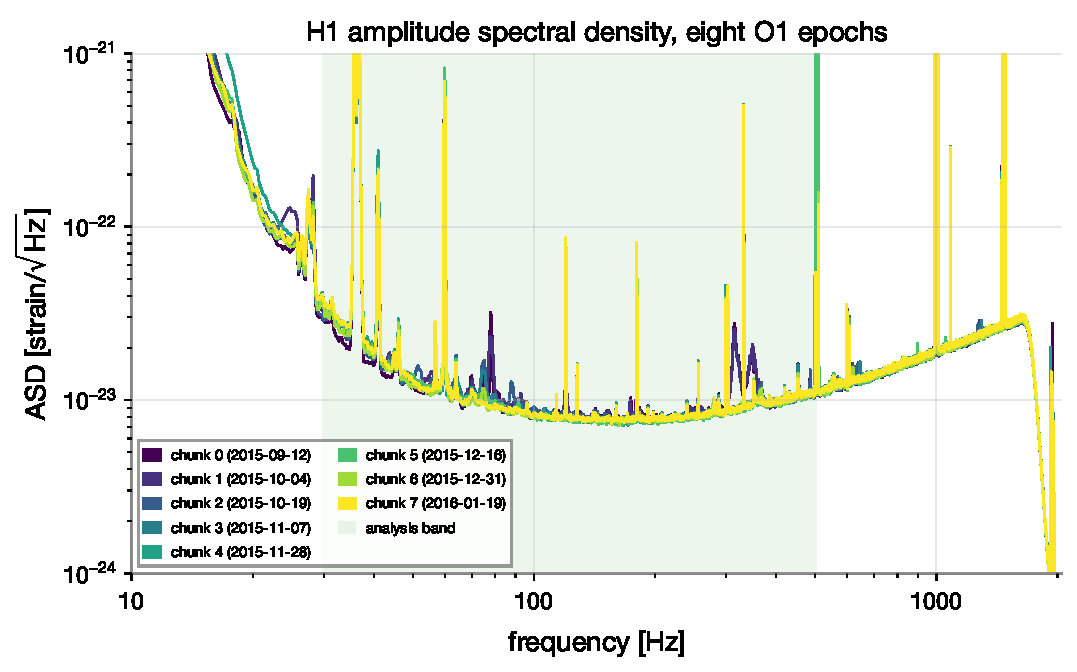
\includegraphics[width=0.62\textwidth]{fig01_asd_chunks.pdf}\hfill
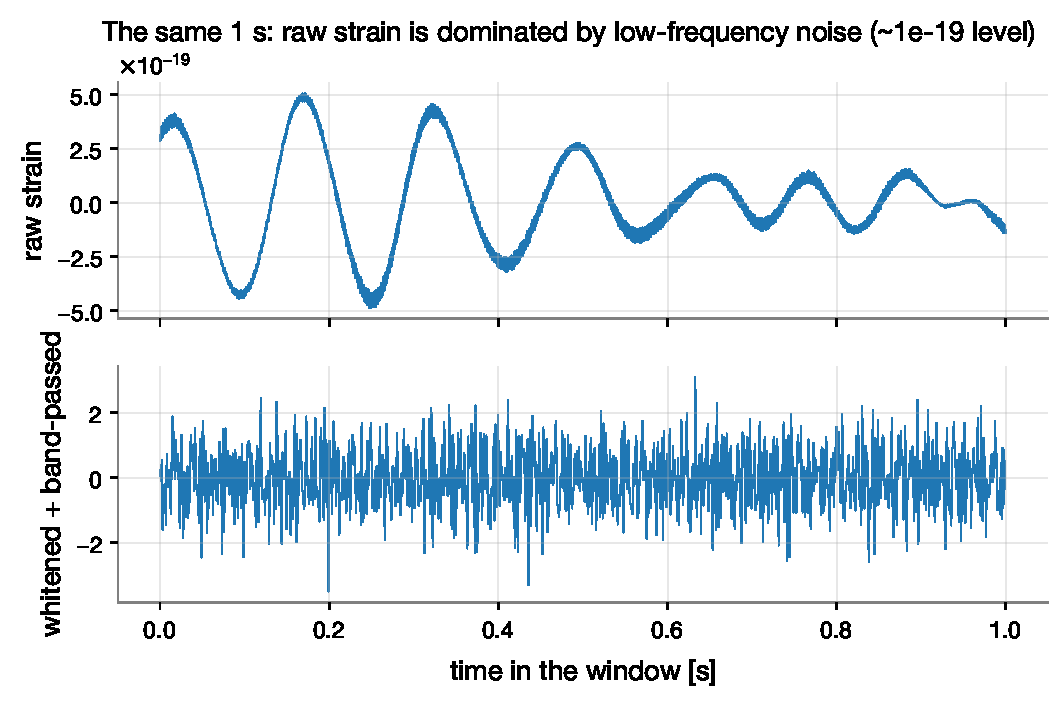
\includegraphics[width=0.36\textwidth]{fig01_raw_vs_white.pdf}
\caption{Left: ASD of the eight chunks. Right: the same second of data, raw and whitened (the raw strain is dominated by low-frequency noise).}\label{fig:asd}
\end{figure}

\subsection{How Gaussian and stationary is the noise?}
The likelihood used in Sections~\ref{sec:freq} and~\ref{sec:bayes} assumes independent standard-normal whitened bins. We test it against a Gaussian reference built with the same chain
from ideal bins (Figure~\ref{fig:gauss}):
\begin{itemize}[nosep]
\item \textbf{Bulk.} The sample distribution follows $\mathcal N(0,1)$ down to a probability of $\sim10^{-4}$; the bin variance is $2$ (the expected value) within a few per cent in the quiet epochs, and the correlation between adjacent bins is $0.012$, at the level of the statistical floor.
\item \textbf{Lines and non-stationarity.} The bin variance dips at the 60\,Hz harmonics (the median-Welch PSD slightly over-estimates narrow lines at 1\,Hz resolution) and shows broad excess power in the glitchier epochs (chunks 4 and 6).
\item \textbf{Tails.} A fraction $10^{-4}$ of the samples lies beyond $5\sigma$ (Gaussian: $6\times10^{-7}$) and the loudest windows reach hundreds of $\sigma$; the plain standard deviation of chunk 6 is $1.8$ against a robust $\sigma$ of $0.95$.
Chunk 2 is exceptional: $3.5\,\%$ of its windows exceed the Gaussian 99.9th percentile of the window energy and the lag-1 autocorrelation of the window energy is $0.80$ (long glitchy stretches).
\end{itemize}
These are the glitches and the non-stationarity of the real detector. They are the reason why \emph{every} threshold in this report is set on real background, and why calibration is always tested on chunks that were not used to set it.

\begin{figure}[h]\centering
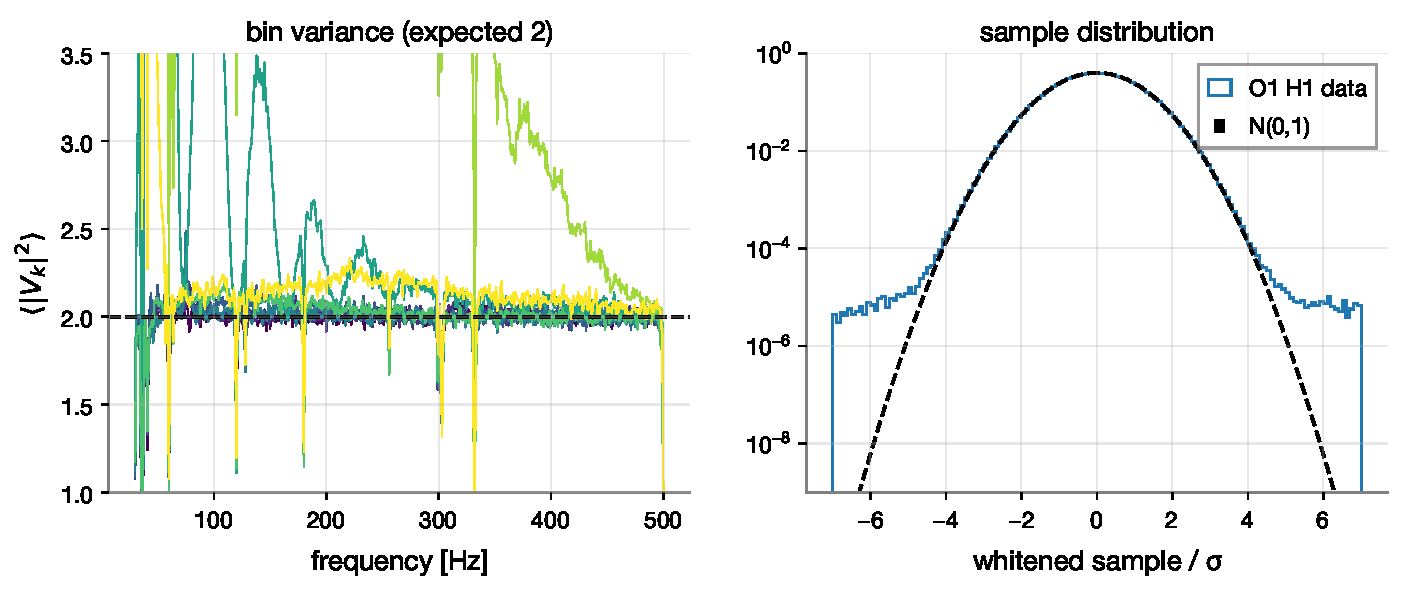
\includegraphics[width=0.95\textwidth]{fig01_gaussianity.pdf}\\[0.3em]
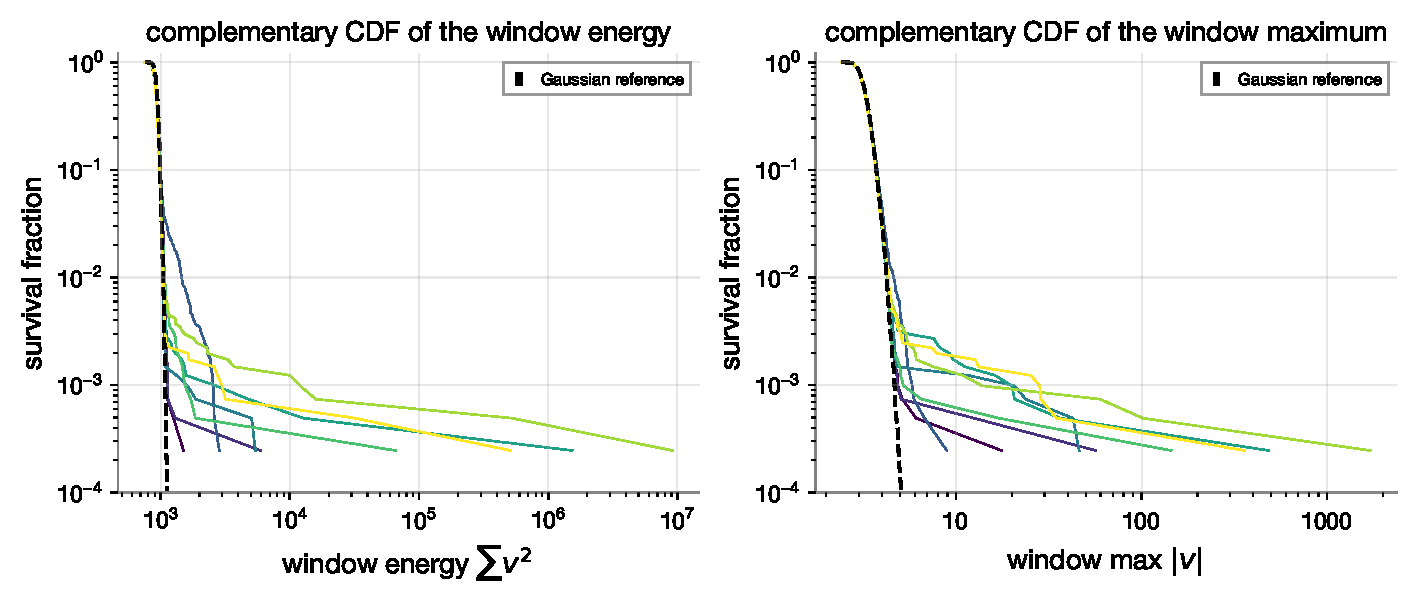
\includegraphics[width=0.95\textwidth]{fig01_window_tails.pdf}
\caption{Top: bin variance of each chunk (left; the expected value is~2) and distribution of the whitened samples against $\mathcal N(0,1)$ (right). Bottom: complementary distribution of the window energy and of the window maximum for each chunk against the Gaussian reference (dashed).}\label{fig:gauss}
\end{figure}
